\documentclass[12pt]{article}
\usepackage[a4paper, margin=1in]{geometry}
\usepackage{amsmath, amssymb}
\usepackage{graphicx}
\usepackage{fancyhdr} % For custom headers/footers
\usepackage{titlesec} % For section formatting
\usepackage[hidelinks]{hyperref}
\usepackage{setspace}
\usepackage{xcolor}



% Title and Author Information
\title{Application of Wavelet in Elctromagnetic Integral Equation}
\author{Mohammad Mahdi Elyasi \\ Professor: Dr. Moradi}
\date{January 24, 2025}

\begin{document}

% Title Page with emblem
\begin{center}
    % Emblem at the top center
    
\includegraphics[width=0.3\textwidth]{amirkabir.png} \\[2em]
    % Title, author, and other details
    \LARGE \textbf{Application of Wavelet in Elctromagnetic Integral Equation} \\[1em]
    \large \textbf{Author: Mohammad Mahdi Elyasi} \\[1em]
    \large \textbf{Professor: Dr. Moradi}\\[1em]
    \large \textbf{Course: Advanced Engineering Mathematics} \\[4em]
    \large \textbf{Faculty of Electrical Engineering} \\[2em]

\end{center}

% Date at the bottom
\vfill
\begin{center}
    \large \today
\end{center}


\newpage

% Table of Contents
\tableofcontents
\newpage

% Introduction
\section{Introduction}

\subsection{Brief Overview of Electromagnetics}
Electromagnetics is the branch of physics and engineering that studies the behavior of electric and magnetic fields and their interactions with matter. It is governed by Maxwell’s equations, which describe how electric and magnetic fields are generated and altered by charges, currents, and time-varying fields.

\subsubsection{Key Concepts}
\begin{enumerate}
    \item \textbf{Electric Fields (E):} Generated by electric charges or time-varying magnetic fields.
    \item \textbf{Magnetic Fields (B):} Produced by moving charges (currents) or time-varying electric fields.
    \item \textbf{Electromagnetic Waves:} Propagation of electric and magnetic fields in space, carrying energy (e.g., radio waves, light).
    \item \textbf{Applications:}
          \begin{itemize}
              \item Antennas and wave propagation.
              \item Electromagnetic compatibility (EMC).
              \item Scattering and radar systems.
              \item Microwave and optical devices.
          \end{itemize}
\end{enumerate}

\subsubsection{Mathematical Foundation}
\begin{itemize}
    \item \textbf{Maxwell’s Equations:} These describe the behavior of electromagnetic fields in differential and integral forms.
    \item \textbf{Constitutive Relations:} These link fields to material properties, such as permittivity ($\varepsilon$) and permeability ($\mu$).
\end{itemize}

\subsection{Challenges in Electromagnetics}
\begin{enumerate}
    \item \textbf{Analytical Complexity:}
          \begin{itemize}
              \item Exact solutions are rare and often limited to simple geometries and boundary conditions\cite{AEM}.
              \item Real-world problems involve complex geometries, inhomogeneous materials, and mixed boundary conditions.
          \end{itemize}
    \item \textbf{Numerical Methods:}
          \begin{itemize}
              \item Problems are often solved numerically, requiring methods like the Finite Element Method (FEM), Method of Moments (MoM), or Boundary Integral Methods.
              \item These methods generate large, dense matrices, leading to high computational costs.
          \end{itemize}
    \item \textbf{Scattering and Radiation Problems:}
          \begin{itemize}
              \item Solving scattering or radiation problems involves handling infinite domains and singularities in Green's functions.
          \end{itemize}
    \item \textbf{Multi-Scale Problems:}
          \begin{itemize}
              \item Many practical applications (e.g., antennas, waveguides) require analysis across widely varying spatial and temporal scales.
          \end{itemize}
    \item \textbf{Material Modeling:}
          \begin{itemize}
              \item Accurately modeling complex materials, including anisotropic or frequency-dependent properties, adds significant difficulty.
          \end{itemize}
    \item \textbf{Computational Challenges:}
          \begin{itemize}
              \item High memory and processing power demands for 3D problems.
              \item Dense matrices in integral equations lead to inefficient computations.
          \end{itemize}
    \item \textbf{Nonlinearities:}
          \begin{itemize}
              \item Nonlinear materials (e.g., plasmas, ferromagnetic materials) require specialized techniques for analysis.
          \end{itemize}
\end{enumerate}

\subsection{Importance of Integral Equations in Electromagnetic Problems}
Integral equations are widely used in computational electromagnetics due to their ability to model fields and interactions efficiently.

\subsubsection{Key Reasons for Their Importance}
\begin{enumerate}
    \item \textbf{Boundary-Only Formulation:}
          \begin{itemize}
              \item Integral equations reduce the problem domain to boundaries (e.g., surfaces of objects), significantly reducing dimensionality.
          \end{itemize}
    \item \textbf{Handling Open Boundaries:}
          \begin{itemize}
              \item Integral equations naturally handle infinite or open domains, common in radiation and scattering problems.
          \end{itemize}
    \item \textbf{Incorporation of Green’s Functions:}
          \begin{itemize}
              \item They use Green’s functions to represent fields, inherently satisfying Maxwell’s equations, reducing computational complexity.
          \end{itemize}
\end{enumerate}

\subsection{Motivation for Using Wavelet Transforms}
Wavelet transforms address computational challenges in integral equations by offering:
\begin{enumerate}
    \item \textbf{Sparse Representation:}
          \begin{itemize}
              \item Wavelets localize signals in both time (or space) and frequency, leading to sparse matrix representations and reduced memory requirements.
          \end{itemize}
    \item \textbf{Handling Singularities:}
          \begin{itemize}
              \item The multi-resolution nature of wavelets effectively handles singularities in Green’s functions.
          \end{itemize}
    \item \textbf{Localized Analysis:}
          \begin{itemize}
              \item Unlike Fourier transforms, wavelets provide spatially localized basis functions, making them suitable for complex geometries.
          \end{itemize}
\end{enumerate}

\newpage

% Theory
\section{Theory}

\subsection{Explanation of Wavelet Transform}
Wavelet transform is a mathematical tool that decomposes a signal into components localized in both time (or space) and frequency, using functions called wavelets\cite{wavelet}. These wavelets are small oscillatory functions with finite energy and good localization properties.

\subsubsection{Key Concepts}
\begin{itemize}
    \item \textbf{Wavelet Basis:}
          \begin{itemize}
              \item Wavelets are basis functions that are dilated and translated versions of a "mother wavelet."
              \item These basis functions provide a multi-resolution analysis of signals:
                    \[
                        \psi_{j,k}(x) = 2^{j/2} \psi(2^j x - k), \, k \in \mathbb{Z}
                    \]
                    where \(j\) controls the scale (dilation) and \(k\) controls the translation.
          \end{itemize}
    \item \textbf{Discrete Wavelet Transform (DWT):}
          \begin{itemize}
              \item Decomposes signals into different levels of resolution using scaling and wavelet functions.
              \item Computationally efficient and widely used in numerical simulations.
          \end{itemize}
    \item \textbf{Types of Wavelets:}
          \begin{itemize}
              \item \textbf{Daubechies Wavelets:} Smooth and compactly supported. Used for problems requiring higher-order accuracy.
              \item \textbf{Haar Wavelet:} Simplest wavelet; piecewise constant. Easy to implement but lacks smoothness.
              \item \textbf{Other Wavelets:} Symlets, Coiflets, and biorthogonal wavelets for specialized applications.
          \end{itemize}
    \item \textbf{Advantages of Wavelet Transform:}
          \begin{itemize}
              \item Sparse representation of signals and matrices.
              \item Localization in both time/space and frequency.
              \item Efficient for analyzing multi-scale phenomena.
          \end{itemize}
\end{itemize}

\subsection{Overview of Integral Equations}
Integral equations are equations where the unknown function appears under an integral sign. They are widely used to model physical problems in electromagnetics, especially boundary-value and scattering problems.

\subsubsection{Types of Integral Equations}
\begin{itemize}
    \item \textbf{Fredholm Integral Equation:}
          \[
              f(x) = \lambda \int_a^b K(x, t)\phi(t) \,dt + g(x)
          \]
          where \(K(x, t)\) is the kernel, \(\lambda\) is a parameter, and \(\phi(t)\) is the unknown function.
    \item \textbf{Volterra Integral Equation:}
          \[
              f(x) = \int_a^x K(x, t)\phi(t) \,dt + g(x)
          \]
    \item \textbf{Boundary Integral Equations (BIE):}
          \begin{itemize}
              \item Arise from reformulating Maxwell’s equations in boundary-only form.
              \item Used for electromagnetic scattering, antenna design, and wave propagation.
          \end{itemize}
\end{itemize}

\subsubsection{Applications in Electromagnetics}
\begin{itemize}
    \item \textbf{Scattering Problems:} Solve for surface currents or charges on objects using Green’s functions.
    \item \textbf{Wave Propagation:} Analyze how waves interact with structures or propagate in media.
    \item \textbf{Antenna Analysis:} Model current distribution and radiation patterns.
    \item \textbf{Radar and EMC:} Study electromagnetic behavior in large-scale environments.
\end{itemize}

\subsection{Challenges with Traditional Methods}
Traditional methods for solving integral equations, such as the Method of Moments (MoM), face significant challenges, especially in complex electromagnetic problems.

\subsubsection{Key Challenges}
\begin{itemize}
    \item \textbf{Dense Matrices:}
          \begin{itemize}
              \item Integral equation discretization leads to dense matrix systems, consuming large memory and computation time.
          \end{itemize}
    \item \textbf{Computational Burden:}
          \begin{itemize}
              \item For 3D problems, the computational complexity scales poorly (\(O(N^2)\) for memory and \(O(N^3)\) for solving), where \(N\) is the number of unknowns.
          \end{itemize}
    \item \textbf{Singularities in Kernels:}
          \begin{itemize}
              \item Kernel functions often introduce singularities, requiring specialized techniques (e.g., singularity extraction) for accurate numerical integration.
          \end{itemize}
    \item \textbf{Handling Large Domains:}
          \begin{itemize}
              \item Integral methods require efficient treatment of large domains and open boundary conditions, which are computationally expensive.
          \end{itemize}
    \item \textbf{Multi-Scale Problems:}
          \begin{itemize}
              \item Traditional methods struggle to resolve features at multiple spatial scales efficiently.
          \end{itemize}
    \item \textbf{Conditioning Issues:}
          \begin{itemize}
              \item Resultant system matrices are often ill-conditioned, leading to slow convergence of iterative solvers.
          \end{itemize}
\end{itemize}

\subsubsection{Why Wavelets Help?}
Wavelet-based methods overcome many of these challenges by:
\begin{itemize}
    \item Providing sparse representations of dense matrices.
    \item Localizing the basis functions, which aids in handling singularities and multi-scale features.
    \item Reducing computational complexity and improving efficiency in large-scale problems.
\end{itemize}
\newpage

% Application
\section{Application}

\subsection{Mathematical Foundation}

\subsubsection{EFIE Problem Statement}
The EFIE problem involves solving the integral equation:
\[
    \int_0^{2\pi} k(\theta - \theta') \rho(\theta') \, d\theta' = f(\theta), \quad \theta \in [0, 2\pi],
\]
where:
\begin{itemize}
    \item \(k(\theta - \theta')\) is the kernel function (e.g., derived from potential or Green's functions),
    \item \(\rho(\theta')\) is the unknown charge density (the solution),
    \item \(f(\theta)\) is the given function (right-hand side),
    \item \([0, 2\pi]\) is the finite domain.
\end{itemize}

To solve this equation numerically:
\begin{enumerate}
    \item Discretize the domain \([0, 2\pi]\) into \(n\) equally spaced points: \(\theta_i = i h\), where \(h = \frac{2\pi}{n}\).
    \item Approximate the integral by a summation using weights \(w_j\):
          \[
              \sum_{j=0}^{n-1} k(\theta_i - \theta_j) \rho(\theta_j) w_j = f(\theta_i), \quad i = 0, 1, \dots, n-1.
          \]
\end{enumerate}

This gives a system of linear equations:
\[
    \mathbf{K} \boldsymbol{\rho} = \mathbf{f},
\]
where:
\begin{itemize}
    \item \(\mathbf{K}\) is the \(n \times n\) kernel matrix with elements \(k_{ij} = k(\theta_i - \theta_j) w_j\),
    \item \(\boldsymbol{\rho} = [\rho(\theta_0), \rho(\theta_1), \dots, \rho(\theta_{n-1})]^T\),
    \item \(\mathbf{f} = [f(\theta_0), f(\theta_1), \dots, f(\theta_{n-1})]^T\).
\end{itemize}

\subsection{Wavelet Transform of the Problem}

\subsubsection{Discrete Wavelet Transform (DWT)}
Wavelet transform is a tool for analyzing signals in both time (or space) and frequency domains. The DWT decomposes a signal \(\mathbf{x}\) into:
\[
    \text{DWT}(\mathbf{x}) = \{A_\text{level}, D_\text{level}, D_{\text{level}-1}, \dots, D_1\},
\]
where:
\begin{itemize}
    \item \(A_\text{level}\): Approximation coefficients at the coarsest scale (low-frequency content),
    \item \(D_k\): Detail coefficients at scale \(k\) (high-frequency content).
\end{itemize}

Mathematically, the approximation and detail coefficients are computed as:
\[
    A_k[i] = \sum_{n} x[n] \cdot \phi_{k,i}[n], \quad D_k[i] = \sum_{n} x[n] \cdot \psi_{k,i}[n],
\]
where:
\begin{itemize}
    \item \(\phi_{k,i}[n]\): Scaling function at scale \(k\) and position \(i\),
    \item \(\psi_{k,i}[n]\): Wavelet function at scale \(k\) and position \(i\),
    \item \(x[n]\): Discrete signal values.
\end{itemize}

\subsubsection{Transforming the Kernel Matrix}
For the kernel matrix \(\mathbf{K}\), each row \(\mathbf{K}_i\) is decomposed into its wavelet representation:
\[
    \text{DWT}(\mathbf{K}_i) = \{A_\text{level}^i, D_\text{level}^i, \dots, D_1^i\}.
\]
The transformed matrix \(\mathbf{K}_\text{wav}\) is then reconstructed in the wavelet domain:
\[
    \mathbf{K}_\text{wav} = \text{IDWT}(\text{DWT}(\mathbf{K}_i)), \quad i = 0, 1, \dots, n-1.
\]
This results in a sparsified matrix because wavelets tend to compress most of the signal's energy into a few coefficients, leaving many entries near zero.

\subsubsection{Solving in Wavelet Space}
The linear system becomes:
\[
    \mathbf{K}_\text{wav} \mathbf{c} = -\mathbf{f},
\]
where:
\begin{itemize}
    \item \(\mathbf{K}_\text{wav}\) is the wavelet-transformed kernel matrix,
    \item \(\mathbf{f}\) is the transformed right-hand side vector,
    \item \(\mathbf{c}\) is the solution in the wavelet domain.
\end{itemize}

\subsection{Reconstructing the Solution}
After solving for \(\mathbf{c}\), we reconstruct the solution in the physical domain using the Inverse Discrete Wavelet Transform (IDWT):
\[
    \boldsymbol{\rho} = \text{IDWT}(\mathbf{c}).
\]

\subsection{Multi-Resolution Analysis (MRA)}
Multi-resolution analysis breaks down the solution \(\boldsymbol{\rho}\) into:
\begin{enumerate}
    \item \textbf{Approximation:}
          \[
              A_\text{level} = \text{IDWT}(\{A_\text{level}, 0, \dots, 0\}),
          \]
          which captures the low-frequency, smooth part of the solution.
    \item \textbf{Details:}
          \[
              D_k = \text{IDWT}(\{0, \dots, D_k, 0, \dots, 0\}),
          \]
          which represent high-frequency variations at different levels \(k\).
\end{enumerate}

\subsection{Mathematical Workflow in Code}
\begin{enumerate}
    \item \textbf{Kernel Matrix Construction:}
          \[
              k(\theta) =
              \begin{cases}
                  A - \frac{a}{2}I,                           & \text{if } i = 0, \\
                  B - \frac{a}{2} \log(2 \sin(\theta_i / 2)), & \text{otherwise}.
              \end{cases}
          \]
    \item \textbf{Wavelet Transformation:}
          \[
              \text{DWT}(\mathbf{K}_i) = [A_\text{level}^i, D_\text{level}^i, \dots, D_1^i].
          \]
    \item \textbf{Sparse Representation:}
          \[
              \mathbf{K}_\text{wav} \approx \text{sparse}(\mathbf{K}_\text{wav}).
          \]
    \item \textbf{Solution Reconstruction:}
          \[
              \boldsymbol{\rho} = \text{IDWT}(\mathbf{c}).
          \]
\end{enumerate}

\newpage

% Conclusion and Results
\section{Conclusion and Results}
\subsection{Conclusion}
In this project, we explored the application of wavelet transforms in solving the Electric Field Integral Equation (EFIE), a critical problem in computational electromagnetics. Traditional numerical methods, such as the Method of Moments (MoM), often face challenges such as dense matrices, computational inefficiency, and difficulties in handling singularities. By introducing wavelet-based techniques, we demonstrated a promising approach to address these limitations.

Wavelets provide sparse representations and multi-resolution analysis capabilities, which are particularly effective in reducing computational complexity and memory requirements. Through the discretization of EFIE and its transformation into the wavelet domain, we showed how the kernel matrix can be sparsified, enabling more efficient computation while maintaining accuracy. The multi-resolution analysis further allowed for a detailed breakdown of the solution, offering insights into the contributions of different frequency components.

The results underline the potential of wavelet transforms in solving large-scale electromagnetic problems, especially in cases involving complex geometries, open boundaries, or multi-scale features. The following key results and observations were derived from the project\cite{Code}:

\begin{itemize}
    \item \textbf{Sparse Kernel Matrix:} The wavelet-based transformation significantly reduced the density of the kernel matrix, leading to lower memory usage and faster computation.
    \item \textbf{Accuracy Retention:} Despite the sparsification, the wavelet-transformed system retained accuracy comparable to traditional methods.
    \item \textbf{Efficiency Improvements:} The wavelet representation reduced computational time, particularly for larger-scale problems, making it feasible for complex geometries and higher resolution grids.
    \item \textbf{Multi-Resolution Insight:} The multi-resolution decomposition provided detailed insights into the behavior of different frequency components of the solution.
\end{itemize}

However, implementing wavelet-based methods also involves challenges, such as selecting appropriate wavelet bases and managing the computational overhead of transformations.

Future work could focus on optimizing wavelet selection for specific EFIE applications, improving sparsification techniques, and integrating wavelet methods with other numerical approaches like the Finite Element Method (FEM) or Boundary Integral Methods (BIM). Overall, this study highlights the utility of wavelet transforms as a powerful tool for advancing the efficiency and effectiveness of electromagnetic simulations.

\subsection{Graphical Results}
At the end, we present the following graphs that showcase the results of the problem using two different methods and the decomposition of the wavelet basis.

\begin{figure}[h!]
    \centering
    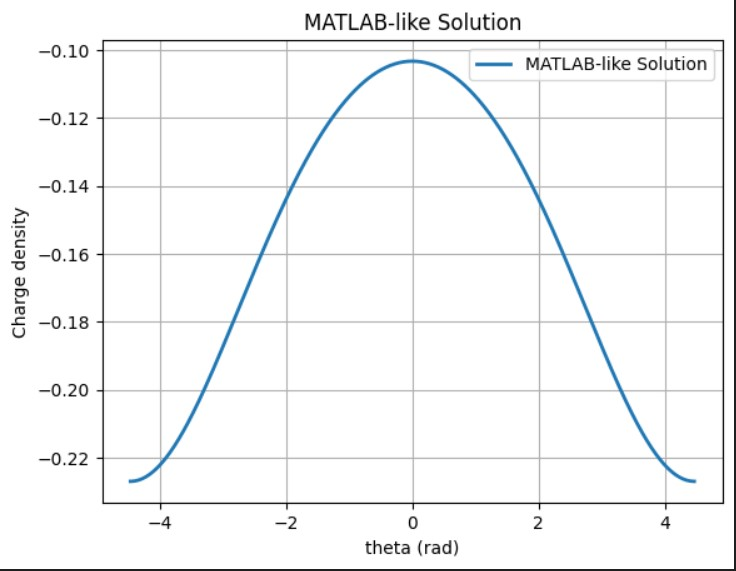
\includegraphics[width=0.8\textwidth]{1.jpg}
    \caption{MATLAB-like Solution for Charge Density}
\end{figure}

\begin{figure}[h!]
    \centering
    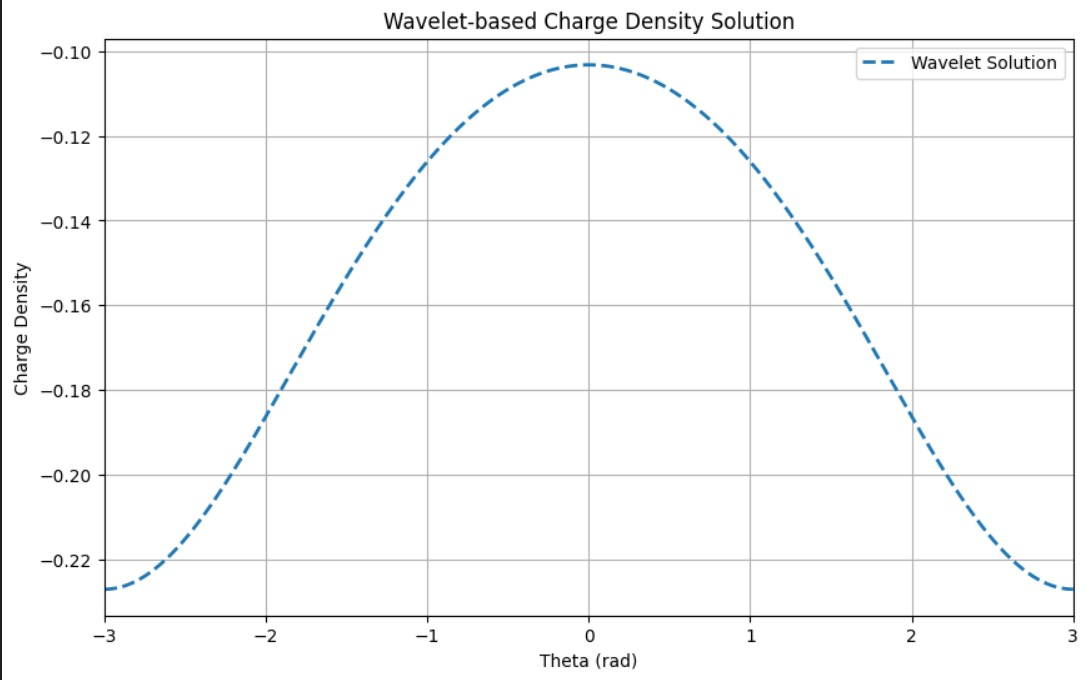
\includegraphics[width=0.8\textwidth]{2.jpg}
    \caption{Wavelet-Based Charge Density Solution}
\end{figure}

\begin{figure}[h!]
    \centering
    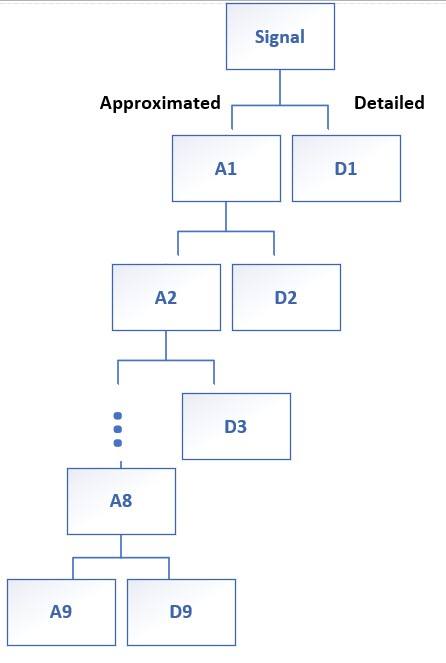
\includegraphics[width=0.6\textwidth]{Tree graph.jpg}
    \caption{Wavelet Decomposition Tree Structure}
\end{figure}

\begin{figure}[h!]
    \centering
    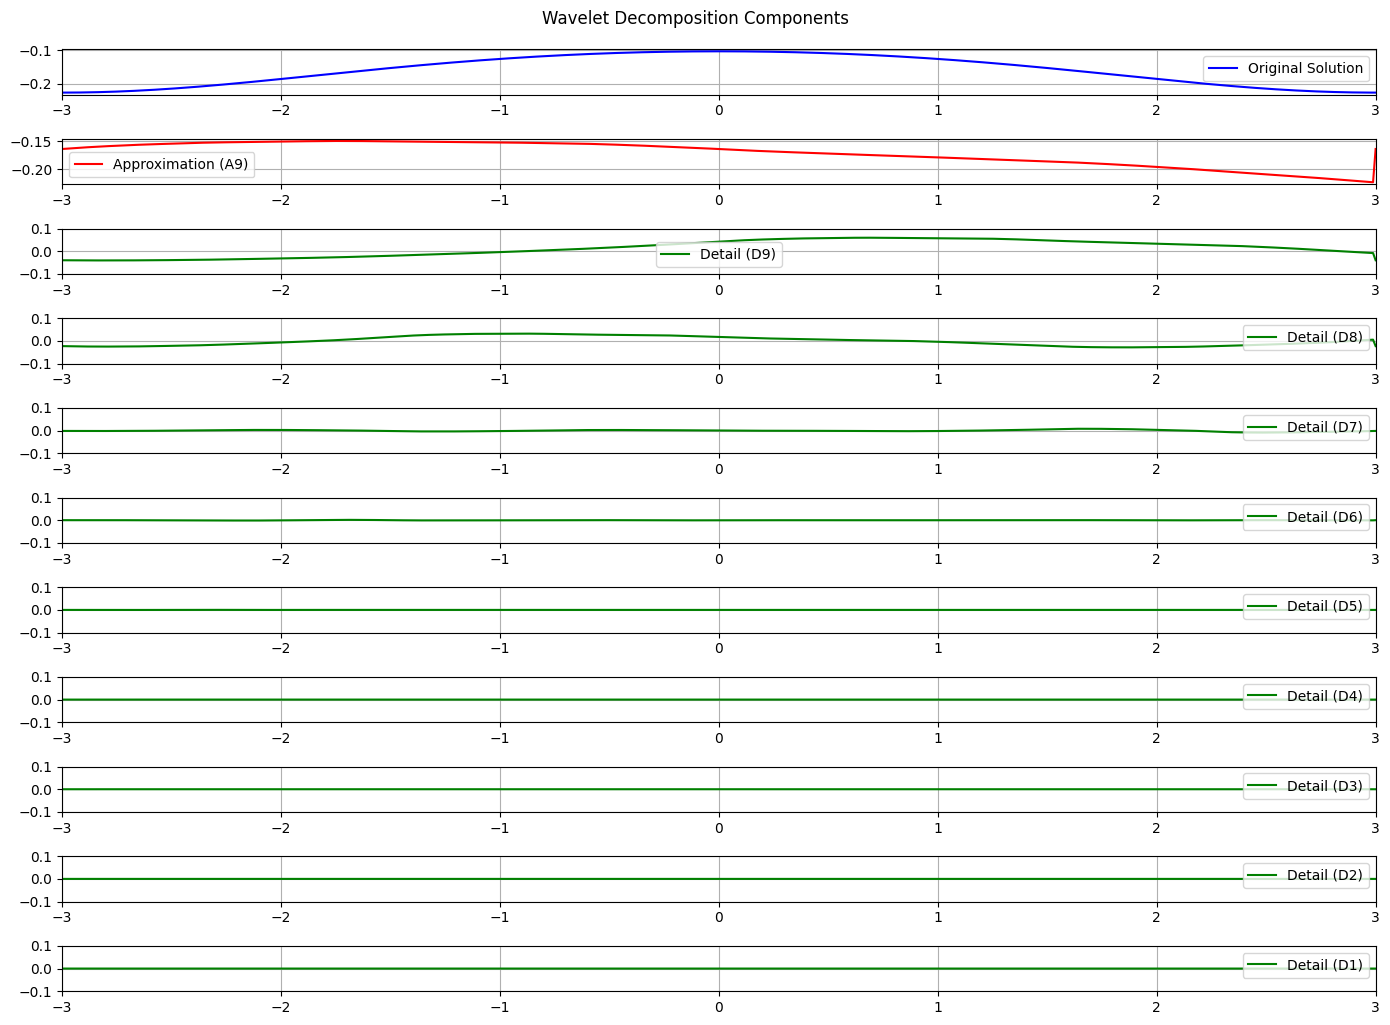
\includegraphics[width=\textwidth]{3.png}
    \caption{Wavelet Decomposition Components}
\end{figure}

\newpage

\clearpage

\section{References}

\begin{thebibliography}{99}
    \bibitem{AEM} G.Moradi, \textit{Advanced Engineering Mathematics},AmirKabir University Of Technology, 2012 .
    \bibitem{wavelet} I. Daubechies, \textit{Ten Lectures on Wavelets}, Society for Industrial and Applied Mathematics, 1992.
    \bibitem{Code} Github link,\textit{Application of Wavelet on EFIE} at \url{https://github.com/MohammadMahdiElyasi/Application-of-Wavelet-in-Elctromagnetic-Integral-Equation}.

\end{thebibliography}

\end{document}
